% !TEX program = pdflatex

%%%%%%%%%%%%%%%%%%%%
%affineConway.tex
%%%%%%%%%%%%%%%%%%%%%

\pdfoutput=1 %When you use pdflatex
\documentclass{amsart} %When you use pdflatex
\renewcommand{\baselinestretch}{1.2}

\usepackage{tikz}

\usepackage{amssymb}
\usepackage{amsmath}
\usepackage{url}
\usepackage{bm}
\usepackage{enumitem}
\usepackage{graphicx}

\usepackage{hyperref}
\hypersetup{
 colorlinks = true,
 linkcolor = blue,
 filecolor = blue,
 urlcolor = blue,
 citecolor = blue,
}
\hypersetup{unicode=true}

%\input mymacros.tex
%%%%%%%%%%%%%%%%%%%%%%%%%%%%%%%%%%%%%%%%%%%%
%
%   MY MACROS: start 2025 Aug 12
%
%%%%%%%%%%%%%%%%%%%%%%%%%%%%%%%%%%%%%%%%%%%%%

% erase: for temporarily removing text from output
\newcommand{\erase}[1]{}

% ----- Theorem-like environments -----
% Plain style: italic body, bold heading
\theoremstyle{plain}
\newtheorem{theorem}{Theorem}[section]       % Main theorem environment
\newtheorem{lemma}[theorem]{Lemma}           % Lemma, shares numbering with theorem
\newtheorem{proposition}[theorem]{Proposition} % Proposition, shares numbering
\newtheorem{corollary}[theorem]{Corollary}   % Corollary, shares numbering

% Definition style: upright body, bold heading
\theoremstyle{definition}
\newtheorem{definition}[theorem]{Definition} % Definition, shares numbering
\newtheorem{example}[theorem]{Example}       % Example
\newtheorem{algorithm}[theorem]{Algorithm}   % Algorithm description
\newtheorem{claim}[theorem]{Claim}           % Claim
\newtheorem{construction}[theorem]{Construction} % Construction

% Remark style: upright body, italic heading
\theoremstyle{remark}
\newtheorem{remark}[theorem]{Remark}         % Remark

% Number equations, tables, and figures by section
\numberwithin{equation}{section}
\numberwithin{table}{section}
\numberwithin{figure}{section}

% Change QED symbol for end of proof
\newcommand{\qedbox}{\hfill {$\Box$}}

% ----- FONT SHORTCUTS -----
% Blackboard bold (mathbb)
\newcommand{\bbA}{\mathord{\mathbb{A}}}
\newcommand{\BB}{\mathord{\mathbb{B}}}
\newcommand{\CC}{\mathord{\mathbb{C}}}
\newcommand{\DD}{\mathord{\mathbb{D}}}
\newcommand{\EE}{\mathord{\mathbb{E}}}
\newcommand{\FF}{\mathord{\mathbb{F}}}
\newcommand{\GG}{\mathord{\mathbb{G}}}
\newcommand{\HH}{\mathord{\mathbb{H}}}
\newcommand{\II}{\mathord{\mathbb{I}}}
\newcommand{\JJ}{\mathord{\mathbb{J}}}
\newcommand{\KK}{\mathord{\mathbb{K}}}
\newcommand{\LL}{\mathord{\mathbb{L}}}
\newcommand{\MM}{\mathord{\mathbb{M}}}
\newcommand{\NN}{\mathord{\mathbb{N}}}
\newcommand{\OO}{\mathord{\mathbb{O}}}
\newcommand{\PP}{\mathord{\mathbb{P}}}
\newcommand{\QQ}{\mathord{\mathbb{Q}}}
\newcommand{\RR}{\mathord{\mathbb{R}}}
\newcommand{\bbSS}{\mathord{\mathbb{S}}}
\newcommand{\TT}{\mathord{\mathbb{T}}}
\newcommand{\UU}{\mathord{\mathbb{U}}}
\newcommand{\VV}{\mathord{\mathbb{V}}}
\newcommand{\WW}{\mathord{\mathbb{W}}}
\newcommand{\XX}{\mathord{\mathbb{X}}}
\newcommand{\YY}{\mathord{\mathbb{Y}}}
\newcommand{\ZZ}{\mathord{\mathbb{Z}}}

% Calligraphic letters (mathcal)
\newcommand{\AAA}{\mathord{\mathcal{A}}}
\newcommand{\BBB}{\mathord{\mathcal{B}}}
\newcommand{\CCC}{\mathord{\mathcal{C}}}
\newcommand{\DDD}{\mathord{\mathcal{D}}}
\newcommand{\EEE}{\mathord{\mathcal{E}}}
\newcommand{\FFF}{\mathord{\mathcal{F}}}
\newcommand{\GGG}{\mathord{\mathcal{G}}}
\newcommand{\HHH}{\mathord{\mathcal{H}}}
\newcommand{\III}{\mathord{\mathcal{I}}}
\newcommand{\JJJ}{\mathord{\mathcal{J}}}
\newcommand{\KKK}{\mathord{\mathcal{K}}}
\newcommand{\LLL}{\mathord{\mathcal{L}}}
\newcommand{\MMM}{\mathord{\mathcal{M}}}
\newcommand{\NNN}{\mathord{\mathcal{N}}}
\newcommand{\OOO}{\mathord{\mathcal{O}}}
\newcommand{\PPP}{\mathord{\mathcal{P}}}
\newcommand{\QQQ}{\mathord{\mathcal{Q}}}
\newcommand{\RRR}{\mathord{\mathcal{R}}}
\newcommand{\SSS}{\mathord{\mathcal{S}}}
\newcommand{\TTT}{\mathord{\mathcal{T}}}
\newcommand{\UUU}{\mathord{\mathcal{U}}}
\newcommand{\VVV}{\mathord{\mathcal{V}}}
\newcommand{\WWW}{\mathord{\mathcal{W}}}
\newcommand{\XXX}{\mathord{\mathcal{X}}}
\newcommand{\YYY}{\mathord{\mathcal{Y}}}
\newcommand{\ZZZ}{\mathord{\mathcal{Z}}}


% Fraktur letters (mathfrak)
\newcommand{\SSSS}{\mathord{\mathfrak{S}}}    % Symmetric group symbol
\newcommand{\AAAA}{\mathord{\mathfrak{A}}}    % Alternating group symbol

%For vectors
\newcommand{\vect}[1]{\boldsymbol{#1}}

% ----- ARROWS -----

%ARROWS

\newcommand{\maprightsp}[1]{\xrightarrow{\smash{#1}}}
\newcommand{\mapleftsp}[1]{\xleftarrow{\smash{#1}}}
\newcommand{\maprightsb}[1]{\xrightarrow[\smash{#1}]{}}
\newcommand{\maplefts}[1]{\xleftarrow[\smash{#1}]{}}

\newcommand{\inj}{\hookrightarrow}
\providecommand{\twoheadrightarrow}{\mathrel{\rightarrow\!\!\!\!\rightarrow}}
\newcommand{\surj}{\twoheadrightarrow}

\newcommand{\isom}{\xrightarrow{\raise -3pt \hbox{\scriptsize $\sim$} }}


% Vertical arrows
\newcommand{\mapdown}{\mathrel{\downarrow}}
\newcommand{\mapdownleft}[1]{\mathrel{\llap{\scriptstyle#1\;}\downarrow}}


% ----- SET NOTATION -----
\newcommand{\set}[2]{\{\,{#1}\mid {#2} \,\}}           % { x | condition }
\newcommand{\bigset}[2]{\left\{\; {#1} \; \left\vert \; {#2} \;  \right.\right \}}
\newcommand{\bigsetR}[2]{\left\{\; \left. {#1} \; \right\vert \; {#2} \;  \right \}}

\newcommand{\angs}[1]{\langle {#1}  \rangle}           % < x >


% ----- COMMON SYMBOLS -----
\newcommand{\wt}{\widetilde}
\newcommand{\ol}{\overline}
\newcommand{\tensor}{\otimes}
\newcommand{\inv}{^{-1}}                 % superscript -1
\newcommand{\dual}{^{\vee}}               % dual vector space
\newcommand{\comp}{^{\wedge}}             % complement or wedge power

% Primes and related notations
\newcommand{\pprime}{\prime\prime}
\newcommand{\sprime}{^{\prime}}
\newcommand{\sprimeinv}{^{\prime-1}}
\newcommand{\spar}[1]{^{(#1)}}
\newcommand{\spprime}{^{\prime\prime}}
\newcommand{\spcirc}{^{\mathord{\circ}}}
\newcommand{\sptimes}{^{\times}}
\newcommand{\sperp}{^{\perp}}

% Group theory and algebra notation
\newcommand{\fiberproduct}{\Box}            % fibre product symbol
\newcommand{\semidirectproduct}{\rtimes}    % semidirect product
\newcommand{\semidirectproductrev}{\ltimes} 

% Boundary and derivative
\newcommand{\bdr}{\partial\,}
\newcommand{\der}{\partial}

% Math operators (upright text in math mode)
\DeclareMathOperator{\Aut}{Aut}
\DeclareMathOperator{\Image}{Im}
\DeclareMathOperator{\Sing}{Sing}
\DeclareMathOperator{\Spec}{Spec}
\DeclareMathOperator{\Stab}{Stab}
\DeclareMathOperator{\Ker}{Ker}
\DeclareMathOperator{\Coker}{Coker}
\DeclareMathOperator{\Gal}{Gal}
\DeclareMathOperator{\Hom}{Hom}
\DeclareMathOperator{\rank}{rank}
\DeclareMathOperator{\pr}{pr}
\DeclareMathOperator{\disc}{disc}
\DeclareMathOperator{\sgn}{sgn}
\DeclareMathOperator{\characteristic}{char}
\DeclareMathOperator{\length}{leng} % 'leng' probably intended as 'length'

% Sheaf Hom
\newcommand{\sheafHom}{\mathord{\mathcal {Hom}}}

% Classical groups
\newcommand{\GL}{\mathord{\mathrm{GL}}}
\newcommand{\SL}{\mathord{\mathrm{SL}}}
\newcommand{\PGU}{\mathord{\mathrm{PGU}}}
\newcommand{\PSU}{\mathord{\mathrm{PSU}}}
\newcommand{\PGL}{\mathord{\mathrm{PGL}}}
\newcommand{\PSL}{\mathord{\mathrm{PSL}}}
\newcommand{\OG}{\mathord{\mathrm{O}}}
\newcommand{\UG}{\mathord{\mathrm{U}}}
\newcommand{\SO}{\mathord{\mathrm{SO}}}
\newcommand{\SU}{\mathord{\mathrm{SU}}}

% Identity map
\newcommand{\id}{\mathord{\mathrm{id}}}
\newcommand{\Id}{\mathord{\mathrm{Id}}}

% Common notation shortcuts
\newcommand{\Pt}{\PP^2}                      % Projective plane
\newcommand{\Qbar}{\overline{\QQ}}           % Algebraic closure of Q
\newcommand{\pione}{\pi_1}  % Fundamental group

% Inner product or pairing
\newcommand{\intf}[1]{\langle #1 \rangle}

% Transpose symbol
\newcommand{\transpose}{{}^{\mathrm{T}}}

% Vertical spacing helpers (artificially increase the vertical spacing )
\newcommand{\mystruth}[1]{\phantom{\llap{\vrule height #1}}}
\newcommand{\mystrutd}[1]{\phantom{\llap{\vrule depth #1}}}
\newcommand{\mystruthd}[2]{\phantom{\llap{\vrule  height #1 depth #2}}}



%%%%%%%%%%%%%%%%%%%%%%%%%%%%%%%%%%%%%%%%%%%%
%
%   END OF MY MACROS
%
%%%%%%%%%%%%%%%%%%%%%%%%%%%%%%%%%%%%%%%%%%%%%
%\input mymacrosaffineConway.tex
%%%%%%%%%%%%%%%%%%%%%%%%%%%%%%%%%%%%%%%%%%%%
%
%   MY MACROS: start 
%
%%%%%%%%%%%%%%%%%%%%%%%%%%%%%%%%%%%%%%%%%%%%%

\newcommand{\dotz}{\cdot 0}
\newcommand{\dotinf}{\cdot \infty}
\newcommand{\Invols}{\III}
\newcommand{\Cen}{\mathrm{Cen}}
\newcommand{\Leech}{\Lambda}
\newcommand{\Golay}{\CCC_{24}}
\newcommand{\pig}{\pi_{g}}
\newcommand{\varpigt}{\varpi_{(g, \tau)}}
\newcommand{\vep}{\varepsilon}
\newcommand{\PowOmega}{2^{\Omega}}
\newcommand{\weyl}{\vect{w}}

\newcommand{\IIlat}{\mathrm{II}}
\newcommand{\typeILat}{\mathrm{I}}
\newcommand{\typeIILat}{\mathrm{II}}
\newcommand{\Lts}{L_{26}}
\newcommand{\PPPts}{\PPP_{26}}
\newcommand{\FFFts}{{\FFF}_{26}}
\newcommand{\enrinvol}{\epsilon}

\newcommand{\Sigmatwlv}{\varSigma_{12}}
\newcommand{\Laminated}{\varLambda}
\newcommand{\BW}{\mathrm{BW}}

\newcommand{\tname}[1]{$\mathtt{#1}$}


\newcommand{\Lamsxtn}{\Laminated_{16}}
\newcommand{\barLeech}{\overline{\Leech}}
\newcommand{\compword}[1]{\overline{#1}}

\newcommand{\intfLeech}[1]{\intf{#1}_{\Leech}}
\newcommand{\intfL}[1]{\intf{#1}_{\hskip -1pt L}}
\newcommand{\intfM}[1]{\intf{#1}_{\hskip -1pt M}}
\newcommand{\intfSigma}[1]{\intf{#1}_{\hskip -1pt {\varSigma}}}

\newcommand{\tilgamma}{\tilde{\gamma}}
\newcommand{\tilg}{\tilde{g}}

\newcommand{\LeechRoot}[1]{r(#1)}

\newcommand{\AOG}{\mathord{\mathrm{AO}}}

\newcommand{\ConCham}{\mathord{C}}
\newcommand{\ConChamz}{\ConCham(\weyl_0)}


\newcommand{\walls}{\WWW}
\newcommand{\tilwalls}{\widetilde{\WWW}}
\newcommand{\tilXi}{\widetilde{\Xi}}
\newcommand{\Xitau}{\Xi_{\tau}}
\newcommand{\tilXitau}{\tilXi_{\tau}}

\newcommand{\Lplus}{L_{+}}
\newcommand{\Lminus}{L_{-}}
\newcommand{\qplus}{q_{+}}
\newcommand{\qminus}{q_{-}}
\newcommand{\gplus}{g_{+}}
\newcommand{\gminus}{g_{-}}
\newcommand{\Leechplus}{\Leech_{+}}
\newcommand{\Leechminus}{\Leech_{-}}
\newcommand{\etaplus}{{\eta}_{+}}
\newcommand{\etaminus}{{\eta}_{-}}
\newcommand{\lambdaplus}{{\lambda}_{+}}
\newcommand{\lambdaminus}{{\lambda}_{-}}
\newcommand{\FFFplus}{\FFF_{+}}
\newcommand{\prplus}{\pr_{+}}

\newcommand{\PPPplus}{\PPP_{+}}
\newcommand{\vGam}{\varGamma}
\newcommand{\tilvGam}{\widetilde{\varGamma}}
\newcommand{\vSig}{\varSigma}

\newcommand{\prM}{\pr_M}
\newcommand{\prS}{\pr_S}


\newcommand{\prLplus}{\pr^{L}_{+}}
\newcommand{\prLminus}{\pr^{L}_{-}}
\newcommand{\prLeechplus}{\pr^{\Leech}_{+}}
\newcommand{\prLeechminus}{\pr^{\Leech}_{-}}

\newcommand{\barSigma}{\overline{\Sigma}}

%\newcommand{\tauI}{\tau_{\,\typeILat}}
%\newcommand{\tauII}{\tau_{\,\typeIILat}}
\newcommand{\tauI}{\tau_{120}}
\newcommand{\tauII}{\tau_{135}}
%%%%%%%%%%%%%%%%%%%%%%%%%%%%%%%%%%%%%%%%%%%%
%
%   END OF MY MACROS
%
%%%%%%%%%%%%%%%%%%%%%%%%%%%%%%%%%%%%%%%%%%%%%

%%%%%%%%%%%%%%%%%%%%%%%%%%%%
%
\begin{document}
%
Let $X$ be a $K3$ surface such that the lattice $S_X$ is 
of rank  $11$ with the  Gram matrix 
\[
\mathrm{diag}(2, -2,-2, \dots, -2),
\]
and the period $\omega_X\in T_X\tensor\CC$ is general so that
\[
\OG(T_X, \omega_X)=\{\pm \id\}.
\]
The lattice $S_X$ is isomorphic to $\typeILat_{1, 10}(2)$.
Let $e_0, e_1, \dots, e_{10}$ be the vectors of $\typeILat_{1, 10}$  
such that
\[
\intf{e_0, e_0}=1, \qquad \intf{e_i, e_i}=-1 \quad (i=1, \dots, 10), 
 \qquad \intf{e_i, e_j}=0\quad (i\ne j).
\]
By  Vinberg algorithm,
we see that $\typeILat_{1, 10}$ is generated 
by the vectors 
\[
\begin{array}{ccl}
\alpha_0&=&e_0-e_1-e_2-e_3, \\
\alpha_1&=&e_1-e_2, \\
\dots \\
\alpha_9&=&e_9-e_{10}, \\
\alpha_{10}&=&e_{10}, \\
\alpha_{11}&=&3e_0-e_1-\dots -e_{10}, \\
\end{array}
\]
of norms $-2,-2, \dots, -2,-1,-1$, 
and $\OG(\typeILat_{1, 10}, \PPP)$ is generated by the reflections with respect to these vectors.
%
\begin{figure}
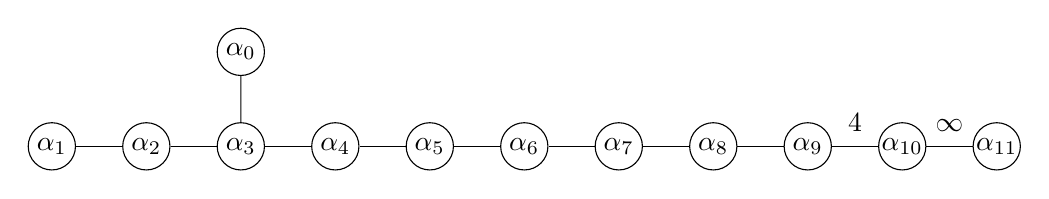
\begin{tikzpicture}[scale =.8, 
  vertex/.style={circle, draw, minimum size=6mm, inner sep=0pt}
]

% vertices
\node[vertex] (a1)  at (0,0)    {$\alpha_1$};
\node[vertex] (a2)  at (1.5,0)  {$\alpha_2$};
\node[vertex] (a3)  at (3,0)    {$\alpha_3$};
\node[vertex] (a4)  at (4.5,0)  {$\alpha_4$};
\node[vertex] (a5)  at (6,0)    {$\alpha_5$};
\node[vertex] (a6)  at (7.5,0)  {$\alpha_6$};
\node[vertex] (a7)  at (9,0)   {$\alpha_7$};
\node[vertex] (a8)  at (10.5,0) {$\alpha_8$};
\node[vertex] (a9)  at (12,0)   {$\alpha_9$};
\node[vertex] (a10) at (13.5,0) {$\alpha_{10}$};
\node[vertex] (a11) at (15,0)   {$\alpha_{11}$};

\node[vertex] (a0) at (3,1.5) {$\alpha_0$};

% edges
\draw (a1) -- (a2);
\draw (a2) -- (a3);
\draw (a3) -- (a4);

\draw (a4) -- (a5);
\draw (a5) -- (a6);
\draw (a6) -- (a7);
\draw (a7) -- (a8);
\draw (a8) -- (a9);

\draw (a9) -- node[above=2pt] {$4$} (a10);
\draw (a10) -- node[above=2pt] {$\infty$} (a11);

\draw (a3) -- (a0);

\end{tikzpicture}
\end{figure}
%
Hence $\OG(S_X, \PPP)$ is also generated  by these $12$ reflections.
The order of $\OG(q_S)$  is 
\[
D:=46998591897600.
\]
The subgroup of $\OG(q_S)$ generated by the image of these $12$ reflections
by the natural homomorphism $\eta_S\colon \OG(S_X, \PPP)\to \OG(q_S)$ is also equal to $D$.
Hence $\eta_S$ is surjective,
and the kernel of $\eta_S$ is is of index $D$ in $ \OG(S_X, \PPP)$.
Note that the discriminant group of $S_X$ is  $2$-elementary, and hence 
the period condition for $g\in  \OG(S_X, \PPP)$ is $\eta_S(g)=\id$.
Therefore we see that the image of
\[
\Aut(X) \to  \OG(S_X, \PPP)
\]
is equal to the subgroup of  the kernel of $\eta_S$
consisting of elements that preserve the nef-and-big cone $N_X$.
%
\newpage
%
\begin{table}
\[
\begin{array}{clrrrr}
\textrm{No.} & \textrm{$ADE$} & \OG(R) & i(\eta_R) & m_2 & m_4 \\
\hline  
1  &  A_{1}+D_{6}  &  64210599936000  &  67456  &  62  &  612  \\ 
2  &  A_{5}  &  133772083200  &  505920  &  30  &  804  \\ 
3  &  A_{1}+A_{3}+D_{4}  &  321052999680  &  2698240  &  38  &  852  \\ 
4  &  3A_{1}+D_{5}  &  535088332800  &  2698240  &  46  &  1028  \\ 
5  &  3A_{1}+D_{4}  &  31708938240  &  4553280  &  30  &  932  \\ 
6  &  3A_{1}  &  127401984  &  5902400  &  6  &  1044  \\ 
7  &  A_{1}+A_{3}  &  707788800  &  6374592  &  14  &  964  \\ 
8  &  11A_{1}+D_{4}  &  2853804441600  &  6475776  &  46  &  772  \\ 
9  &  A_{1}+A_{4}  &  3483648000  &  6475776  &  22  &  1012  \\ 
10  &  A_{2}+A_{3}  &  2090188800  &  6475776  &  18  &  924  \\ 
11  &  5A_{1}+A_{3}  &  9555148800  &  7555072  &  22  &  884  \\ 
12  &  7A_{1}  &  743178240  &  16189440  &  14  &  964  \\ 
13  &  2A_{1}+A_{2}  &  99532800  &  22665216  &  10  &  1004  \\ 
14  &  A_{1}+2A_{2}  &  298598400  &  22665216  &  14  &  1092  \\ 
15  &  15A_{1}  &  67947724800  &  22665216  &  30  &  932  \\ 
16  &  7A_{1}  &  452984832  &  26560800  &  14  &  1092  \\ 
17  &  11A_{1}+D_{4}  &  570760888320  &  32378880  &  46  &  1028  \\ 
18  &  4A_{1}+A_{5}  &  28665446400  &  37775360  &  38  &  1236  \\ 
19  &  5A_{1}+A_{3}  &  1698693120  &  42497280  &  22  &  1012  \\ 
20  &  9A_{1}+D_{6}  &  8561413324800  &  64757760  &  78  &  1476  \\ 
21  &  3A_{1}+2A_{3}  &  5096079360  &  84994560  &  30  &  1188  \\ 
22  &  15A_{1}  &  16307453952  &  94438400  &  30  &  1188  \\ 
23  &  5A_{1}+A_{3}  &  743178240  &  97136640  &  22  &  1140  \\ 
24  &  7A_{1}+2D_{4}  &  1712282664960  &  129515520  &  62  &  1380  \\ 
25  &  11A_{1}+D_{4}  &  67947724800  &  271982592  &  46  &  1284  \\
\end{array}
\]
\caption{Genus of $R$}\label{table:genus}
\end{table}
%
The genus of 
the  orthogonal complement $R=(S_X\inj \Lts)\sperp$ of a primitive embedding $\iota\colon S_X\inj \Lts$  does not depend on
the choice of the embedding $\iota$,
and the mass of this genus is 
\[
\sum_{R} \frac{1}{|\OG(R)|}=\frac{3773551}{128421199872000},
\]
where the summation is taken over a representative set of isomorphism classes in the genus.
By Kneser's neighboring method,
we enumerate all the isomorphism classes of lattices in this genus.
The result is given in Table~\ref{table:genus}.
Here $m_{\nu}$ is the size of $R_{\nu}:=\set{v\in R}{\intf{v,v}=-\nu}$
for $\nu=2, 4$, 
and $ADE$ is the the $ADE$-type of 
the set of roots $R_2$.
The index $i(\eta_R)$ of the image of the natural homomorphism $\eta_R\colon \OG(R)\to \OG(q_R)$ is also presented.
%
\begin{remark}
For the calculation of the sizes of $\OG(R)$,
we used {\tt MAGMA}.
This is my first usage of {\tt MAGMA} (the web calculator).
\end{remark}
%
We say that two primitive embeddings $\iota_1\colon S_X\inj \Lts$ and $\iota_2\colon S_X\inj \Lts$ are equivalent 
if there exist isometries $g_S\colon S_X\cong S_X$ and  $g_L\colon \Lts\cong \Lts$ such that 
$\iota_1  g_L=g_S\iota_2$.
(Note that we write mappings from the right.)
Suppose that we fix a lattice $R$ in the above genus.
Then $q_S$ and $-q_R$ are isomorphic.
Since  the natural homomorphism $\OG(S, \PPP)\to \OG(q_S)$ is surjective,
we see that the action of $\OG(S, \PPP)$ on the set  of isomorphisms $q_S\cong -q_R$ is transitive.
Hence the equivalence  class of primitive embeddings $ S_X\inj \Lts$
is determined solely by  the isomorphism class of 
the orthogonal complement $R=(S_X\inj \Lts)\sperp$.
%
%
\end{document}


